%\documentclass[a4j,twocolumn,uplatex]{jsarticle}
\documentclass[a4j,twocolumn]{jsarticle}

\usepackage[dvipdfmx]{graphicx}
\usepackage{url}
\usepackage{amsmath}
\def\tightlist{\itemsep1pt\parskip0pt\parsep0pt}
\setlength{\textheight}{275mm}
\headheight 5mm
\topmargin -30mm
\textwidth 185mm
\oddsidemargin -15mm
\evensidemargin -15mm
\setlength\textfloatsep{0pt}
\setlength\intextsep{0pt}
\pagestyle{empty}


\begin{document}

\title{command lineによるeditor操作の習熟プログラムの開発}
\author{情報科学科 \hspace{5mm} 27014533 \hspace{5mm} 和田創煕}
\date{}
\maketitle


\section{研究の動機}
最初は西谷によって開発されたshunkuntype(ターミナル上で実行するタイピングソフト)の再開発をテーマにしていたが,タイピングに特化したソフトを開発しても同じようなものがWeb上に大量に配布されており,それ以外の付加価値を付けたソフトを開発しようと考えた.特にeditor操作に関しては
\begin{quotation}
ツールはプログラマ自身の手の延長である.これは他のどのようなソフトウェアツールよりもEditorに対して当てはまる.テキストはプログラミングにおける最も基本的な生素材なので,できる限り簡単に操作できる必要があり,一つの強力なeditorの習熟は作業の効率化に欠かせない\cite{達人プログラマー}. 
\end{quotation}
と記述されている.さらに,西谷研究室ではタイピング,Ruby言語,Emacsによるeditor操作,CUI操作の習熟が作業効率に非常に大きな影響を与えルため習熟を勧めている.そこでこれらの習熟を目的としたソフトを開発しようと考えた.


\section{editor\_learnerの概要}
ソースコードはRuby入門の教科書を参考にしている\cite{ruby}.
\subsection{initialize}
editor\_learnerを動作させた時,最初に自動的に動く部分である.基本的に作業を行うためのファイルの作成,gemでinstallしたeditor\_learnerのパスを格納したインスタンス変数の作成がメインである.
\subsection{random\_check}
開始から終了までの動作の概要は以下の通り,
\begin{enumerate}
\def\labelenumi{\arabic{enumi}.}
\tightlist
\item
用意されたソースコードから1つ選ばれ,question.rbにコピーされ,新しいターミナルが開かれる.
\item
そこでquestion.rbの内容をanswer.rbに写経する.
\item
写経し終えると前のターミナルに戻り"check"とコマンドラインで入力する.
\item
正しければ終了,正しくなければ間違った箇所のみが表示され,再度確認,入力を行い正誤判定の繰り返しをする.
\end{enumerate}
\subsection{sequential\_check}
開始から終了までの動作の概要は以下の通り,
\begin{enumerate}
\def\labelenumi{\arabic{enumi}.}
\tightlist
\item
chapterと問題番号を引数として入力.その問題がq.rbにコピーされる.
\item
その後新しいターミナルが開かれる.
\item
写経し終えた後の動作は2.2の4番からはrandom\_checkと同じ動作である.
\end{enumerate}

\section{他のソフトとの比較}
\begin{table}[h]
\begin{center}
\caption{人気タイピングソフトとeditor\_learnerの利点と欠点とユーザーインタフェース.\label{sample}}
\centering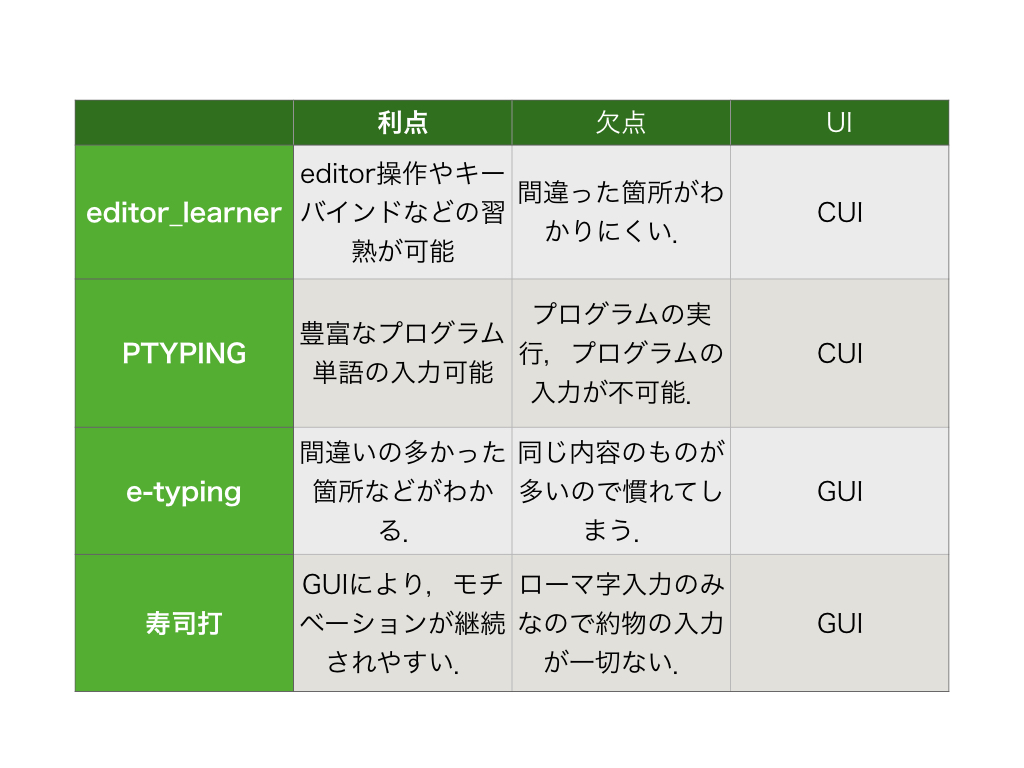
\includegraphics[width=80mm]{../handout/ok/ok.jpeg}
\end{center}

\label{fig:This}
\end{table}
表1は人気タイピングソフトとeditor\_learnerの利点と欠点とユーザーインタフェースを表にしたものである.

CUIに近いPTYPINGが人気の理由はコードに関する単語を入力できるという一点であった.それに加えてeditor\_learnerはeditor操作やコードの入力,実行まで可能になっている.

GUIベースのソフトには継続性に関しては劣る.しかしCUIベースではキーバインド使用により作業の高速化,効率化が期待される.editor\_learnerはプログラマ向けの機能を多数有しているソフトであると言える.

\section{終わりに}
editor\_learnerは\{\}や()など約物の入力やカーソル移動,ファイルの開閉,保存などのCUI操作を全てキーバインドで行う.その結果,editor\_learnerがいかにプログラマ向けのソフトであり,ソフトの目的に沿った技術の向上が期待される.
\begin{thebibliography}{9}
\bibitem{達人プログラマー} Andrew Hunt, David Thomas, 「達人プログラマー」, (オーム社, 2016年).
\bibitem{ruby} 伊藤淳一, 「プロを目指す人のためのRuby入門」, (技術評論社, 2017年)
\end{thebibliography}


\end{document}